\documentclass[11pt]{article}

\usepackage[a4paper,margin=1in]{geometry}
\usepackage{authblk}
\usepackage{booktabs}
\usepackage{graphicx}
\usepackage{hyperref}
\usepackage{microtype}
\usepackage[numbers,super,sort&compress]{natbib}
\usepackage{array}
\usepackage{tabularx}
\usepackage{xcolor}

\hypersetup{
  colorlinks=true,
  linkcolor=black,
  citecolor=black,
  urlcolor=teal
}
\setlength{\parskip}{0.45em}
\setlength{\parindent}{0pt}
\setlength{\emergencystretch}{3em}

\title{\bfseries A Codex-driven closed-loop agent for evidence-gated retrosynthesis planning}

\author[1]{AutoPlanner team}
\affil[1]{AutoPlanner project, local research manuscript draft}
\date{8 June 2026}

\begin{document}
\maketitle

\begin{abstract}
Computer-aided synthesis planning has become increasingly effective at proposing retrosynthetic trees, but practical use is still limited by false route closure, weak provenance for literature-derived transformations and a gap between language-model reasoning and deterministic chemical validation. Here we describe AutoPlanner, a Codex-driven full-flow retrosynthesis agent that uses a large language model as the workflow controller and evidence curator while reserving route acceptance for local validators. Given a target molecule, the system performs deterministic molecular preflight, selects a ChemEnzy-first, literature-first or hybrid workflow, executes ChemEnzy route generation, audits raw routes for stock closure and target identity, extracts literature-backed source-detail transformations, compiles executable one-step rows and emits a final verdict from schema, structure, route and evidence checks. In a hard bufotalin case, the harness rejected 213 raw ChemEnzy routes as fake closures because none passed strict terminal and structural audits. In an atorvastatin endgame case, the same architecture converted two exact literature source-detail steps into executable-ready template rows while preserving a non-solved verdict and blocking production knowledge-base writes. A later strict-visual bufotalin run demonstrates how literature-chain extraction and subgoal closure can be stitched into a solved planner-level route only after validator acceptance. These results show that language-model agents can improve retrosynthesis workflow control without being allowed to fabricate solved chemistry.
\end{abstract}

\textbf{Retrosynthesis planners often fail at the boundary between plausible disconnection and auditable synthesis.} Computer-aided synthesis planning traces back to transform-based synthetic analysis\cite{corey1969retrosynthetic} and has recently advanced through neural reaction prediction, tree search and open-source retrosynthesis systems\cite{segler2018planning,schwaller2020molecular,genheden2020aizynthfinder}. A model may produce a high-scoring route tree, yet the apparent terminal materials can be advanced analogues of the target, the target structure can drift during search, or a literature paragraph can be over-interpreted as an executable transformation. These failure modes are amplified when large language models are used as autonomous chemistry agents\cite{wang2023scientificdiscovery,boiko2023coscientist}: they are useful for source triage, prompt-conditioned planning and structured extraction, but unsafe as final arbiters of route closure.

AutoPlanner addresses this boundary by separating agency from authority. Codex is used as the route-control and open-research agent: it can inspect bounded run artifacts, choose local tools, classify evidence and draft structured candidate artifacts. It cannot mark a target solved, inject raw language-model reactions into production route search, or promote templates to a production knowledge base. Those operations are reserved for deterministic schemas, RDKit structure checks\cite{landrum2024rdkit}, route verifiers, source-detail compilers and final verdict gates.

\section*{Codex-entry route control}

The current AutoPlanner harness begins with a target name, target SMILES and optional family hint (Fig.~\ref{fig:architecture}). A deterministic preflight validates the molecule, computes canonical representations and records risk flags such as steroid-like polycyclic topology. Codex then receives a bounded planning prompt and returns exactly one JSON workflow plan under the \texttt{codex\_entry\_workflow\_plan.v1} schema. The plan must choose one of four strategies: \texttt{chem\_enzy\_first}, \texttt{literature\_first}, \texttt{hybrid} or \texttt{reject\_invalid\_input}. It may schedule only approved local tools.

The default hard-case tool sequence is: run ChemEnzy, audit routes and extract frontiers, run a SMILES-first literature workflow, run the open structure research agent, perform guided ChemEnzy reruns, search route-expansion subgoals, run the self-evolution replay gate, validate the artifact bundle and emit the final verdict. Every run writes an inspectable directory containing the target input, preflight, workflow plan, decision trace, tool-call log, artifact bundle, final verdict and progress panel.

\begin{figure}[t]
  \centering
  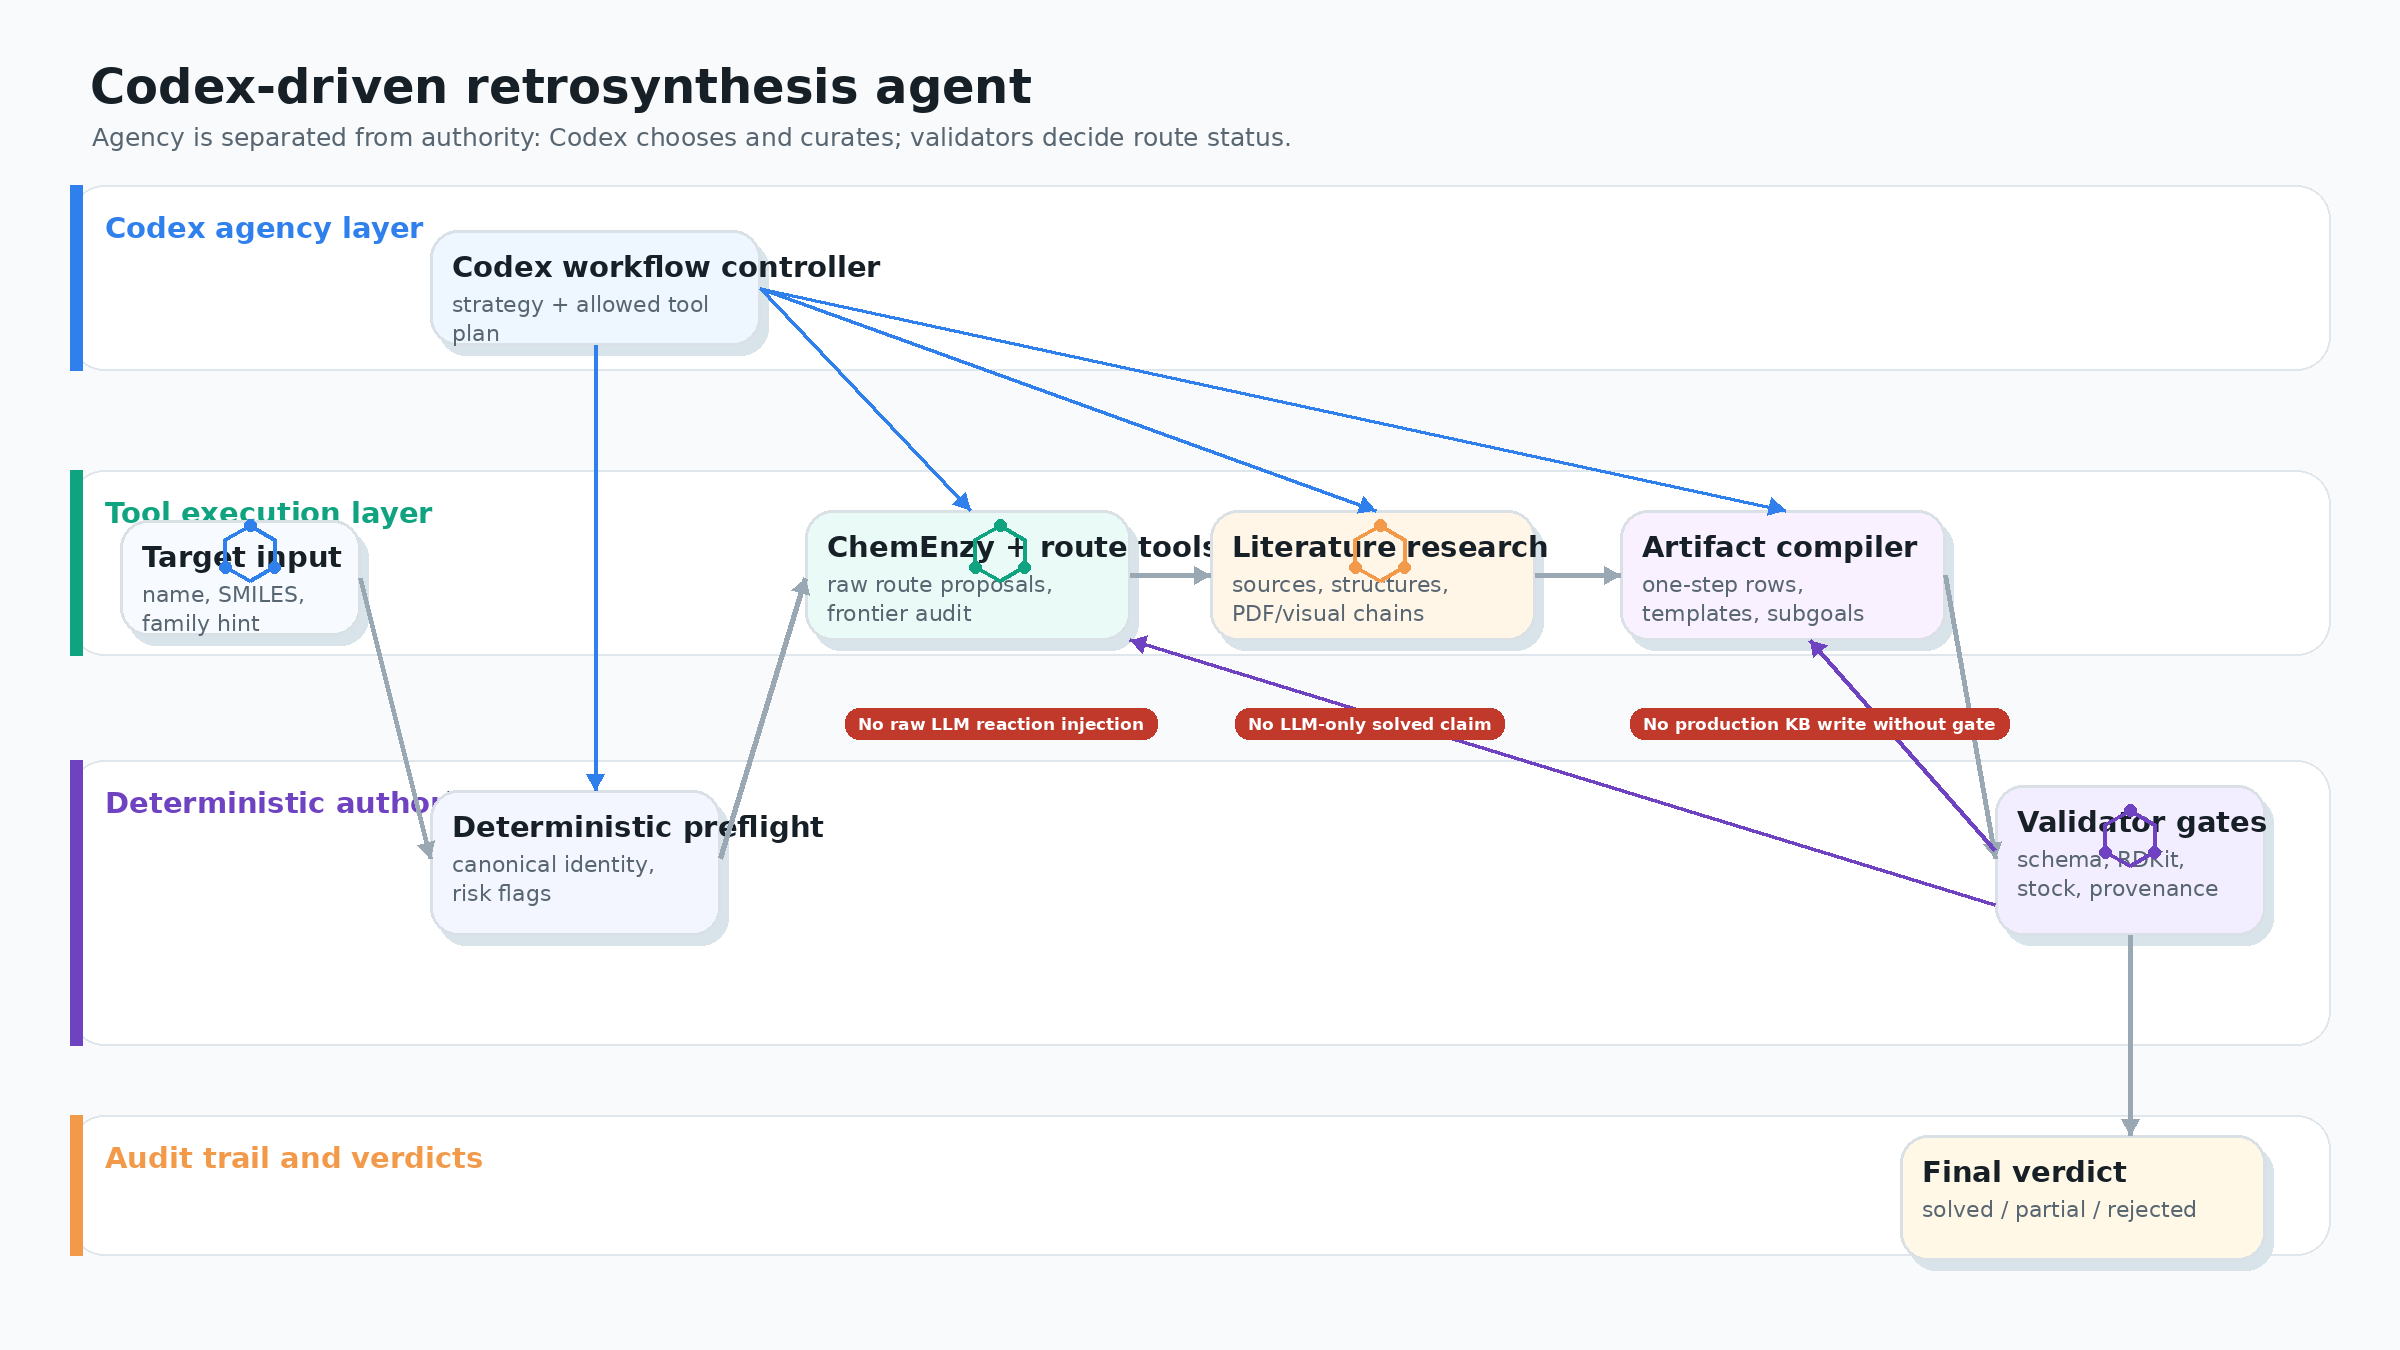
\includegraphics[width=\linewidth]{figures/figure1_architecture.png}
  \caption{\textbf{AutoPlanner full-flow architecture.} The system is organized into four lanes. Codex operates in the agency layer, where it chooses a strategy and schedules only approved tools. Tool execution includes target intake, ChemEnzy route proposal, literature/PDF/visual extraction and downstream artifact compilation. Deterministic authority remains in the preflight and validator gates, which check schema compliance, structure validity, stock closure and provenance before a final verdict is emitted. Red policy labels mark forbidden transitions: raw language-model reaction injection, language-model-only solved claims and production knowledge-base writes without validator approval.}
  \label{fig:architecture}
\end{figure}

The controller is intentionally asymmetric. Codex has broad discretion over which evidence-gathering operation to perform next, but no discretion over final route status. In practice this means that a planned tool can fail or produce only advisory artifacts without corrupting the route state: the failure is written to the audit trail and consumed as feedback for a narrower follow-up run.

\begin{figure}[t]
  \centering
  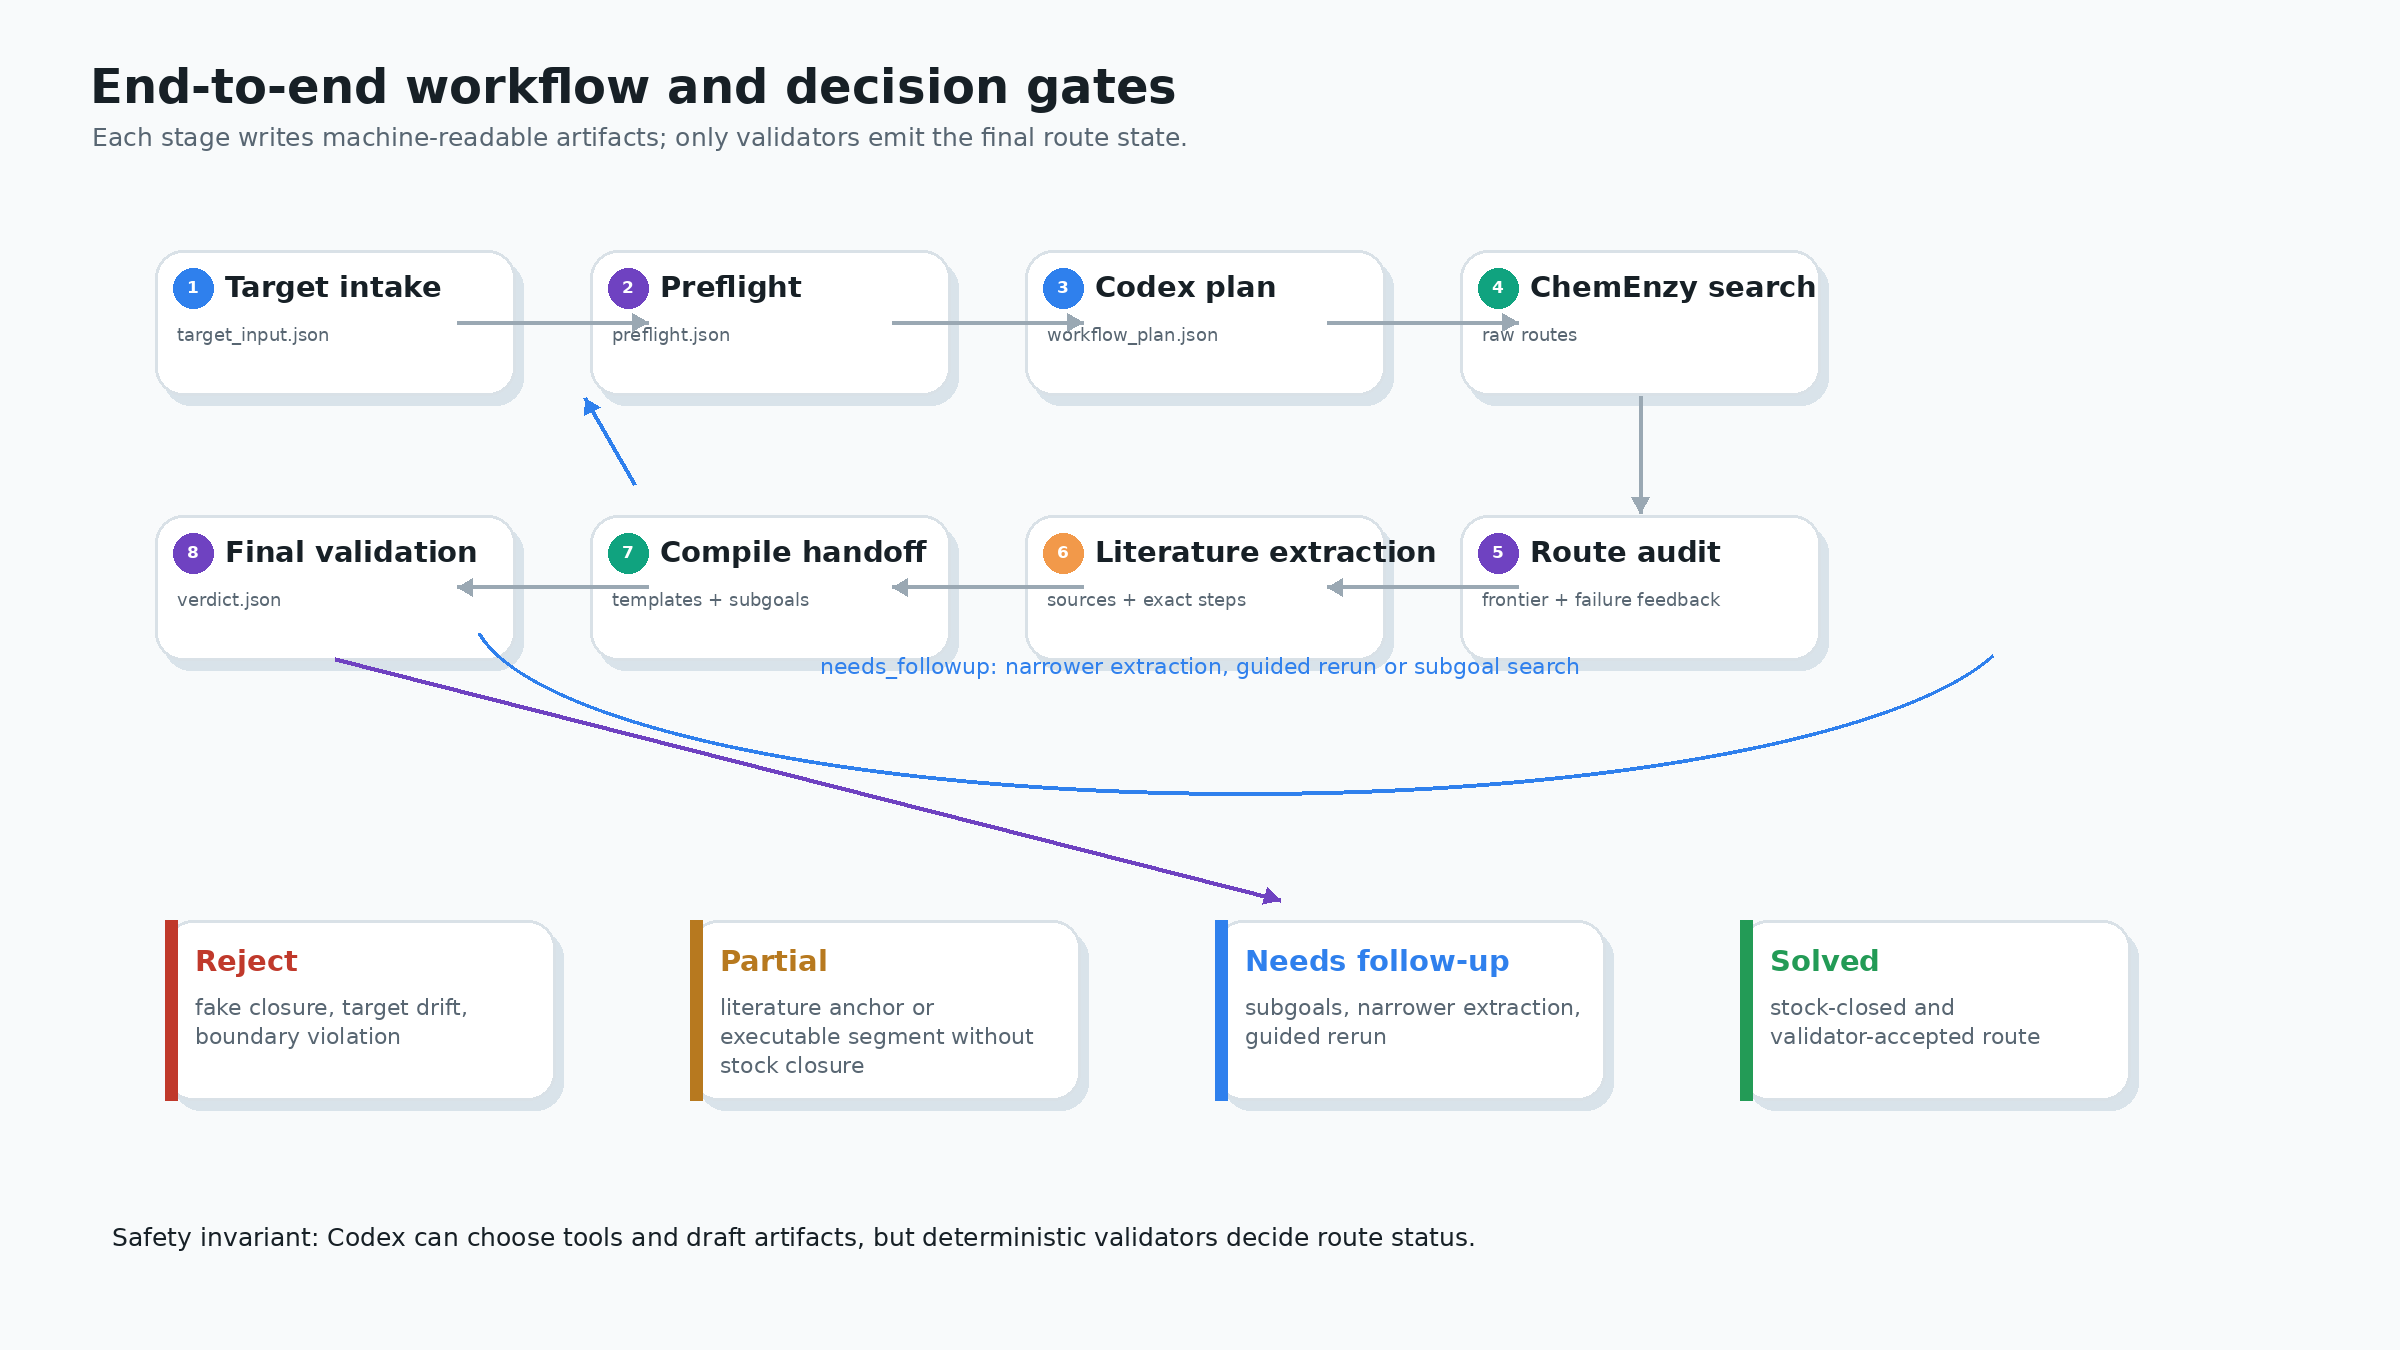
\includegraphics[width=\linewidth]{figures/figure2_workflow_gates.png}
  \caption{\textbf{End-to-end workflow and decision gates.} The default hard-case sequence writes a target input, preflight record, workflow plan, raw route proposals, route audit, literature extraction artifacts, compiled handoff artifacts and a final verdict. Validation can terminate the run as rejected, partial, needs follow-up or solved. The follow-up loop returns to Codex planning with structured failure feedback rather than free-form hidden state.}
  \label{fig:workflow}
\end{figure}

\section*{Route generation as proposal, not authority}

ChemEnzy is treated as a high-value route generator rather than as the final authority. The harness writes the native request and raw result, then audits route claims with a stricter verifier. The verifier checks target equivalence through canonical isomeric SMILES and InChIKey where available, hidden non-stock reactants, large atom jumps, advanced same-scaffold terminal leaves and route-product target matching. The distinction is important: a raw backend flag such as \texttt{solved=true} is evidence that a route generator found a closed tree under its own assumptions, not proof that the route is acceptable under the harness stock and provenance policy.

This design was motivated by steroid and bufadienolide targets. These compounds are prone to fake closure because a route search can terminate at a late-stage same-scaffold precursor that is almost as complex as the target. AutoPlanner therefore records both the route generator result and the verifier result. A route can be useful for diagnosing a frontier while still being rejected for final synthesis planning.

\section*{Literature reasoning under a manifest boundary}

The open research agent is designed to produce downstream-consumable planning assets rather than narrative reports. Each run is governed by an \path{open_research_manifest.json} that binds target identity, route-failure feedback, source order, retrieval boundaries and shell-use policy. Codex may write structured artifacts including structure/template candidates, downstream consumables, literature sources, PubChem-validated compounds and source-detail curator records. It is forbidden to store full procedures, raw reaction strings, unrestricted web dumps or production knowledge-base writes.

The source-detail path converts literature evidence into executable candidates through a deterministic compiler. Curator records must provide product and reactant SMILES, source references, evidence references, exact relation type, product reconstruction status and source-grounded condition metadata. The resolver rejects records that fail RDKit validation, lack source grounding, contain raw reaction strings, request production writes or cannot establish exact reactant-product applicability. Accepted records become one-step rows and literature-template plugin flags; rejected records remain as structured gaps.

\begin{figure}[t]
  \centering
  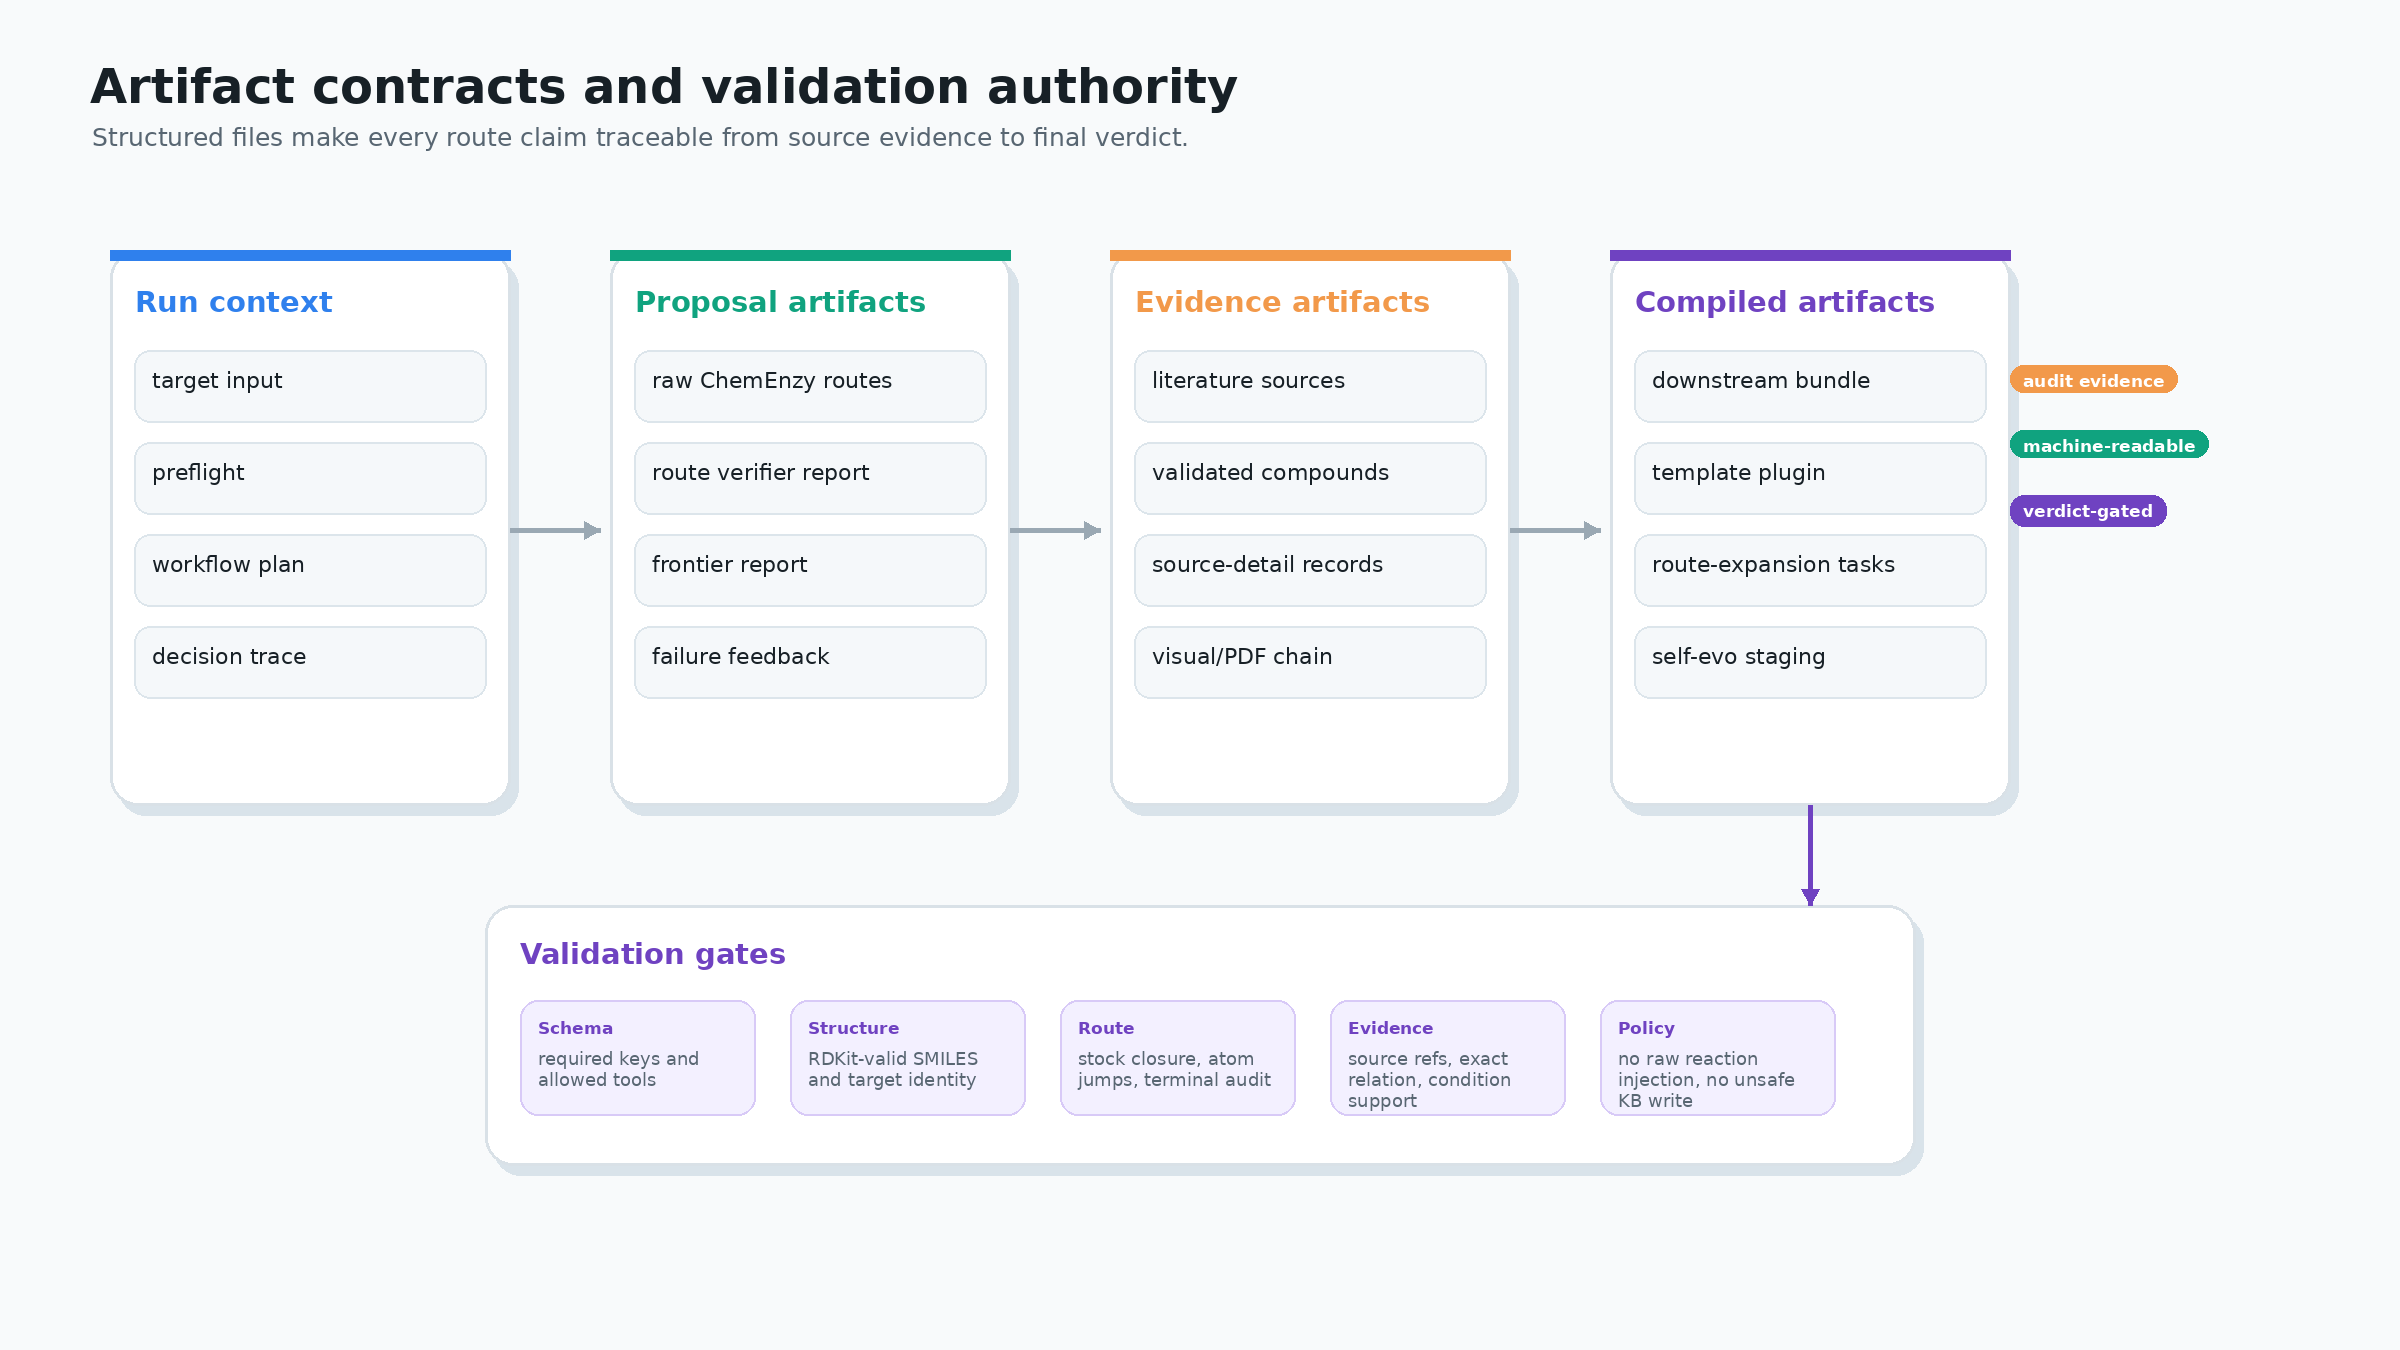
\includegraphics[width=\linewidth]{figures/figure3_artifact_contracts.png}
  \caption{\textbf{Artifact contracts and validation authority.} Run context, proposal artifacts, evidence artifacts and compiled handoff artifacts are serialized as machine-readable files. Validator gates then check required schema fields, RDKit-valid structures, route closure, source evidence and policy constraints. This contract boundary allows Codex to draft and organize evidence while making every route-affecting claim replayable by deterministic code.}
  \label{fig:artifacts}
\end{figure}

\section*{Case study: rejecting false bufotalin closure}

Bufotalin is a stringent test because it combines a polycyclic steroid-like scaffold with a C17 2-pyrone motif and late-stage oxygenation. In the v0 full-flow harness run, the target passed preflight with a steroid-like risk flag. The deterministic offline planner selected a hybrid sequence and executed ChemEnzy with strict building-block stock settings.

ChemEnzy returned 213 raw routes. The verifier accepted zero of them and assigned \path{fake_closed_rejected}: all 213 routes were rejected, with failure reasons including \path{advanced_same_scaffold_terminal}, \path{large_atom_jump} and \path{no_verifier_accepted_stock_closed_route}. The top rejected route had only one step and terminated at a 29-heavy-atom bufotalin-like precursor with target similarity 0.7656. The harness therefore preserved the useful failure signal but blocked the solved claim.

The same run also demonstrates conservative handling of open research. The SMILES-first literature workflow emitted a partial anchor package, but the open structure research tool was rejected because it violated a context boundary by reading a large raw retrieval artifact. Consequently, downstream guided rerun, route expansion and self-evolution production promotion remained blocked. The final verdict was \texttt{fake\_closed\_rejected}, with \texttt{solved=false} and \texttt{stock\_audit\_passed=false}. This is the desired behaviour for a hard target when the evidence is insufficient.

\section*{Case study: compiling atorvastatin literature steps}

Atorvastatin illustrates a different role for the agent: extracting literature-backed transformations without claiming complete synthesis. In the template-extraction demonstration, the open research agent identified exact target and intermediate sources, including PubChem identity anchors and open-access source-detail evidence for an advanced endgame sequence. The deterministic compiler accepted the downstream package, emitted two one-step rows and four template cards, and classified the executable-template maturity as \texttt{executable\_ready}.

The resulting plugin replay returned one candidate for each of the two source-detail steps. The route-expansion handoff contained two child targets and the agent follow-up package contained five actions. The self-evolution replay gate accepted one staging candidate, but production writes remained blocked. The free-acid target replay returned zero full target closures, so the final scientific interpretation remained \texttt{partial\_source\_detail\_segment\_handoff\_not\_solved}: the endgame segment was executable-ready, but stock-to-target synthesis was not solved.

\section*{Stitching literature chains with subgoal closure}

A later bufotalin strict-visual workflow extends the same architecture to PDF and scheme-derived literature chains. The live planner scheduled literature-first tools, including PDF structure extraction, visual chain extraction, intermediate-chain validation, source-detail curator construction, source-detail chain compilation, subgoal search and route stitching. The strict clean verdict for this run was \texttt{solved}, with \texttt{stock\_audit\_passed=true}, after the terminal subgoal request and raw result were accepted by the route-expansion verifier.

This result should be read with the system's evidentiary distinction intact. The literature chain supplies source-detail semisynthetic steps, whereas the terminal subgoal closure is planner-level evidence accepted by the current verifier. The claim is therefore an auditable agent-route closure under the present harness, not an automatically validated laboratory protocol.

\begin{table}[t]
\centering
\caption{\textbf{Representative full-flow outcomes.} Values are taken from local run artifacts generated between 6 and 8 June 2026.}
\label{tab:cases}
\small
\begin{tabularx}{\linewidth}{>{\raggedright\arraybackslash}p{0.17\linewidth}>{\raggedright\arraybackslash}p{0.20\linewidth}>{\raggedright\arraybackslash}p{0.17\linewidth}>{\raggedright\arraybackslash}p{0.22\linewidth}>{\raggedright\arraybackslash}X}
\toprule
Case & Main output & Route count & Accepted rows/routes & Safety outcome \\
\midrule
Bufotalin v0 & fake closure rejected & 213 raw routes & 0 verifier-accepted routes & not solved \\
Atorvastatin endgame & executable-ready segment & partial segment & 2 one-step rows & production writes blocked \\
Bufotalin strict visual & solved planner-level route & terminal subgoal & verifier-accepted closure & stock audit passed \\
\bottomrule
\end{tabularx}
\end{table}

\section*{Discussion}

The main contribution of AutoPlanner is not a new one-step reaction model; it is a control and validation architecture for using language-model agency safely in synthesis planning. Codex is valuable because it can choose between tool workflows, summarize failure feedback, inspect source metadata and turn evidence into structured drafts. The architecture remains scientifically conservative because every route-affecting artifact is filtered by local schemas and validators before it can influence search or verdicts (Figs.~\ref{fig:architecture}--\ref{fig:artifacts}).

The current implementation also exposes its limits. The route verifier can reject advanced same-scaffold terminals and target drift, but it cannot prove laboratory feasibility. Literature extraction can compile exact source-detail rows, but only when reactant and product structures are source-grounded and reconstructable. PDF and visual-chain extraction can recover valuable semisynthetic chains, but mislabelled or missing scheme structures still require strict validation and sometimes narrower prompts. Production self-evolution is intentionally blocked during target runs; staging memory is useful only after replay gates demonstrate that a candidate improves local planning without weakening safety constraints.

These constraints are useful design pressure. A practical retrosynthesis agent should not merely maximize the number of solved flags. It should know when a route is a fake closure, when a literature source is only an advisory anchor, when an extracted step is executable-ready but partial, and when a final solved claim is justified by the verifier. AutoPlanner shows that a Codex-driven agent can make this distinction across full-flow route generation, literature reasoning and subgoal search.

\section*{Methods}

\subsection*{Repository implementation}

The harness entry point is \texttt{scripts/run\_codex\_entry\_controller.py}. Core modules are implemented under \texttt{cascade\_planner/harness/}, including preflight, Codex planning, runner orchestration, tool wrappers, route verification, route-failure feedback, open-research contracts, downstream compilation, source-detail resolution, source-detail chain building, PDF/visual literature extraction, stitched-route validation and self-evolution replay.

\subsection*{Workflow-plan schema}

Codex planning is constrained by \texttt{codex\_entry\_workflow\_plan.v1}. Required fields are schema version, case identifier, recommended strategy, planned tools, rationale, risk flags and expected verdict floor. The allowed tool set is fixed by the harness. Invalid JSON, disallowed tools, missing keys or forbidden chemistry claims cause planner rejection or deterministic fallback.

\subsection*{Deterministic preflight}

Preflight validates target input, canonicalizes SMILES with local cheminformatics tooling and records molecular risk flags. These records are written before Codex planning and become part of the immutable run context. For the bufotalin v0 run, preflight accepted the target, canonicalized the molecule and assigned a polycyclic/steroid-like risk flag.

\subsection*{Route verification}

Raw ChemEnzy output is converted into verifier reports before it can affect final verdicts. The verifier checks route target match, exact target equivalence, terminal-stock status, hidden non-stock leaves, large atom jumps and advanced same-scaffold terminals. Accepted and rejected route counts are reported separately from native backend route counts. Final verdict generation consumes the verifier report rather than raw backend solved flags.

\subsection*{Open-research artifacts}

The open research agent reads \texttt{open\_research\_manifest.json} first and operates within manifest-defined retrieval and context limits. Required artifacts include structure/template candidates, downstream consumables, literature sources, PubChem-validated compounds, validated SMILES and an open-agent audit. Boundary audits detect large raw artifact dumps, forbidden retrieval modes, raw reaction injection and attempted production writes.

\subsection*{Source-detail compilation}

Source-detail curator records are normalized into a resolution pack, merged into downstream consumables and compiled into one-step rows when exact executable candidates exist. A candidate must be source-grounded, RDKit-valid, exact in relation type, structurally reconstructable and accompanied by source-grounded condition metadata. The compiler writes guided ChemEnzy requests, route-expansion tasks, literature-template plugin payloads, executable-template maturity reports, self-evolution staging candidates and follow-up handoff actions.

\subsection*{Self-evolution gate}

Self-evolution is implemented as staging plus replay. Candidate memories can be staged when they pass schema and evidence checks, but target runs keep production writes blocked. Replay reports must show acceptable behaviour before any later promotion path can be considered.

\subsection*{Representative run artifacts}

The bufotalin v0 evidence is stored under \path{results/shared/bufotalin_v0_fullflow_harness_20260606_073155/}. The atorvastatin template-extraction demonstration is stored under \path{results/shared/atorvastatin_template_extraction_demo_20260606/}. The strict-visual bufotalin run is stored under \path{results/shared/bufotalin_fullflow_fresh_visual_existing_pdf_20260608_065053/}. These local artifacts are audit evidence and include final verdicts, route audits, verifier reports, tool-call traces and compiled downstream outputs.

\subsection*{Figure generation}

Figure prompts for a GPT Image 2 architecture background are stored in \path{image2_prompt_architecture.txt}, with the reproducible CLI invocation in \path{generate_image2_architecture.sh}. The current manuscript figures were rendered deterministically with \path{scripts/make_architecture_figures.py} because the local environment did not expose an \path{OPENAI_API_KEY} during drafting. This preserves exact labels and layout while keeping the image-2 prompt ready for replacement with a generated background.

\section*{Data Availability}

The manuscript is generated from the local AutoPlanner repository and local run artifacts. Large run outputs remain under \texttt{results/shared/} and are not intended for blind inclusion in source control. Release packaging should include redacted run summaries, verifier reports, schema definitions and the exact commit hash used for each benchmark table.

\section*{Code Availability}

The relevant code paths are \path{scripts/run_codex_entry_controller.py} and \path{cascade_planner/harness/}. External deployment requires a working ChemEnzy backend, local cheminformatics dependencies and Codex/API credentials configured outside the repository. Production knowledge-base writes are disabled in the reported target runs.

\section*{Acknowledgements}

This draft was generated from AutoPlanner project artifacts. Project-specific funding, institutional and contributor details should be inserted before submission.

\section*{Author Contributions}

The AutoPlanner team designed the harness, implemented the route-control and validation modules, ran the representative workflows and prepared the manuscript draft. Named author contributions should be expanded before submission.

\section*{Competing Interests}

The authors declare no competing interests for this draft.

\bibliographystyle{naturemag}
\bibliography{references}

\end{document}
